\section{Body - defining Bodies}

An INI file can contain an arbitrary number of sections defining bodies. Each body section is opened by \lstinline{[BODY: NAME]} where \lstinline{BODY:} defines the bodies type and \lstinline{NAME} is an unique name to tell different bodies with equal types apart. The \lstinline{order} and the \lstinline{shift_vector} parameters are supported by all bodies but not mandatory. They will be explained later (???TODO ADD REFERENCE???).

\paragraph{Important:} All vectors inside a body section are specified in lattice coordinates by default. For every vector specified in cartesian coordinates the additional parameter \lstinline{someparameter_coordsys} must be added. Its value is either \lstinline{lattice} or \lstinline{cartesian}.

\subsection{Non-periodic bodies}
\subsubsection{Sphere}
The simplest body one can specify is a sphere. The body's section is opened by \lstinline{[sphere: NAME]}. Its size is determined by a  vector pointing from the center of the sphere (at the origin of the coordinate system) to an arbitrary point on its surface.

\paragraph{Parameters}
\begin{description}
 \item{\lstinline{radius_vector}} Vector whose length specifies the radius of the sphere.
\end{description}

\paragraph{Example}\ 

\lstinputlisting{srcexamples/sphere.ini}
\ \\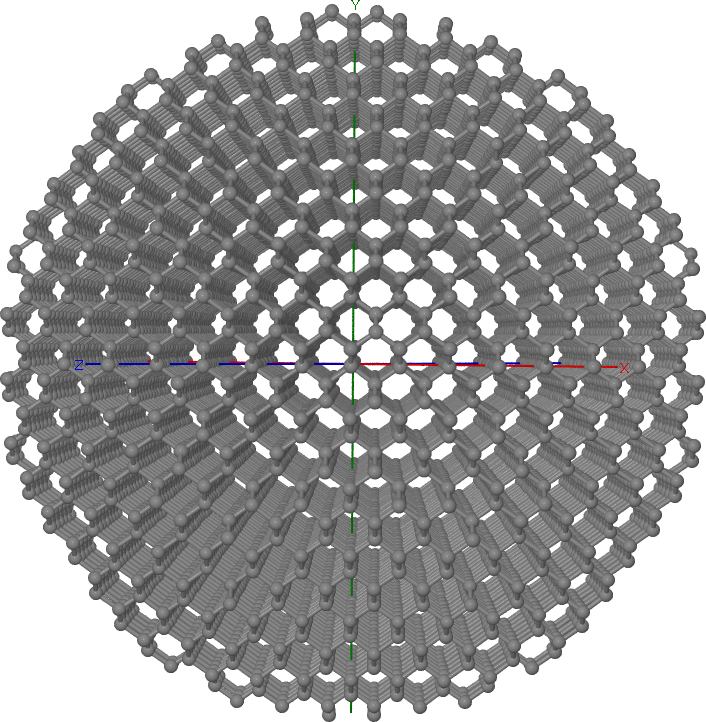
\includegraphics[width=0.6\textwidth]{srcexamples/sphere.png}
\subsubsection{Convex polyhedron}

A convex polyhedron is defined by the planes delimiting the body. A plane can be defined using miller indices or the normal vector. The body's section is opened by \lstinline{[convex_polyhedron: NAME]}.

\paragraph{Parameters}

\begin{description}
 \item{\lstinline{planes_miller}} Miller indices of each plane (except those defined using normal vectors) followed by its distance from the origin.
 \item{\lstinline{planes_normal}} Vector orthogonal to each plane (except those defined using miller indices) followed by its distance from the origin. The vectors do not need to be normalized.
\end{description} 

\paragraph{Example}\

\lstinputlisting{srcexamples/convex_polyhedron.ini}
\ \\\includegraphics[width=0.6\textwidth]{srcexamples/convex_polyhedron.png}
\subsubsection{Cylinder}
In this context, a cylinder is a body with circular base and top areas which are orthogonal to the difference vector of their centers. The edges of base and top area are connected by the smallest lateral area possible. The body's section is opened by \lstinline{[cylinder: NAME]}.

The name ``cylinder'' is a bit misleading, since cylinders and truncated cones are contrivable.

\paragraph{Parameters}
\begin{description}
 \item{\lstinline{point_1}} Position vector to the center of the first circular area.
 \item{\lstinline{radius_1}} Radius of the first circular area.
 \item{\lstinline{point_2}} Position vector to the center of the second circular area.
 \item{\lstinline{radius_2}} Radius of the second circular area.
\end{description}

\paragraph{Example}\ 

\lstinputlisting{srcexamples/cylinder.ini}
\ \\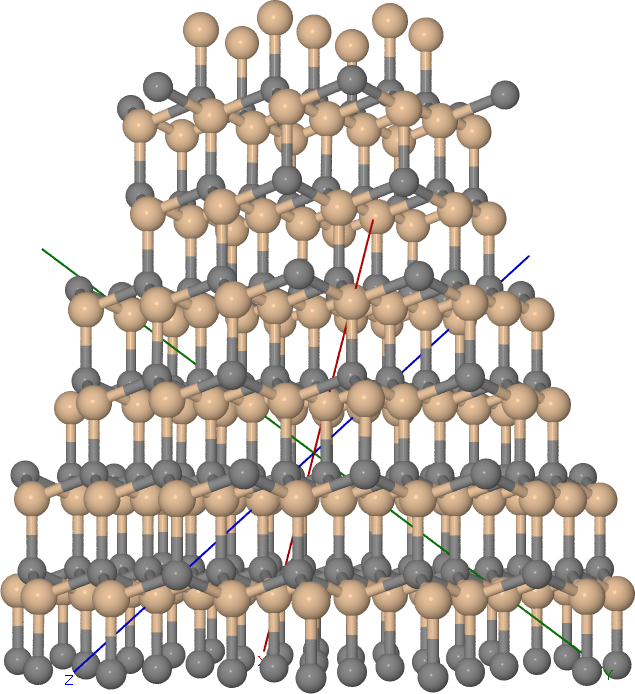
\includegraphics[width=0.6\textwidth]{srcexamples/cylinder.png}
\subsection{1D-periodic bodies}
Apart from the periodity section being a mandatory part of the configuration there is no fundamental difference between creating 1D-periodic structures and non-periodic ones. The resulting supercell is rotated around the origin so that the axis vectors defined in periodicity section it parallel to the z-Axis.

\subsubsection{Periodic Cylinder}
The periodic cylinder is the supercell of an infinitely long cylinder with a circular base area.

\paragraph{Parameters}
\begin{description}
 \item{\lstinline{radius_vector}} Vector whose lenght specifies the radius of the sphere.
\end{description}

\paragraph{Example}\ 

%\lstinputlisting{srcexamples/periodic_1D_cylinder.ini}
???TODO ADD PICTURE OF ....xyz???
\subsubsection{periodic\_1D\_convex\_prism}
\lstinline{periodic_1D_convex_prism} enables cutting a convex prism which can be appended unto itself to create an infinte cut from the given crystal structure. The prism is determined by its surface planes. These planes can be determined in different ways and the combination of planes defined differently is possible. Please note the planes should not surround. They need to lack the base and its projection since these will be calculated to enable the periodicity. The planes should be parallel to the axis or they will be projected accordingly which will change the created body. Of course at least three planes are needed to create a proper body. If no prism can be calculated from the given planes the programm will indicate so and exit.

\paragraph{Parameters}
\lstinline{periodic_1D_convex_prism} requires at least one item of the following. Each item may contain an arbitrary amount of planes each determined by four integer or float values.

\begin{description}
 \item{planes\_miller} \lstinline{planes_miller} contains planes defined by miller indizes. Each plane is given by 4 integers or floats with the first three being the miller indices and the last one the plane's minimum distance from the origin (the length of the smallest possible cartesian vector between the origin and the plane)
 \item{planes\_normal} \lstinline{planes_normal} contains planes defined by a vector orthogonal to the plane and its minimum distance from the origin as in \lstinline{planes_miller}. The vector does not need to be normalized.
\end{description} 

\lstinputlisting{srcexamples/convex_polyhedron}
\lstinputlisting{srcexamples/bodyname}


\subsection{2D-periodic bodies}

Apart from the periodity section being a mandatory part of the configuration there is no fundamental difference between creating 1D-periodic structures and non-periodic ones. The resulting supercell is rotated around the origin so that the z-Axis is orthogonal to both axis vectors defined in the periodicity section.